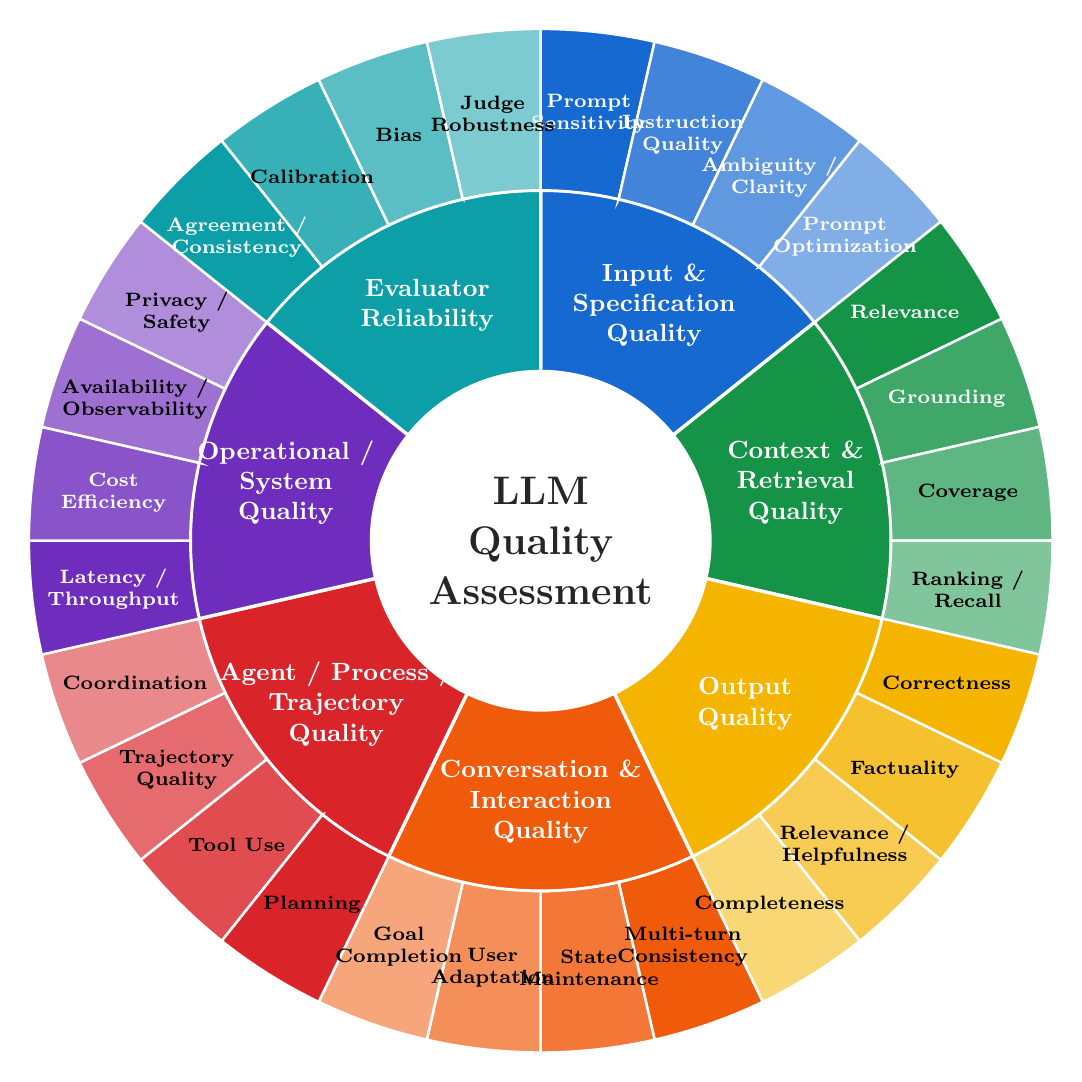
\begin{tikzpicture}[font=\sffamily]
\definecolor{cInput}{HTML}{1769D2}
\definecolor{cContext}{HTML}{159447}
\definecolor{cOutput}{HTML}{F4B400}
\definecolor{cConv}{HTML}{F05A0B}
\definecolor{cAgent}{HTML}{D9252A}
\definecolor{cOps}{HTML}{6F2DBD}
\definecolor{cEval}{HTML}{0C9FA8}

% ---- main ring ----
\foreach \a/\b/\col in {
90/38.5714/cInput,
38.5714/-12.8572/cContext,
-12.8572/-64.2858/cOutput,
-64.2858/-115.7144/cConv,
-115.7144/-167.1430/cAgent,
-167.1430/-218.5716/cOps,
-218.5716/-270/cEval}{
  \path[fill=\col,draw=white,line width=1.2pt]
  (\a:2.15) -- (\a:4.45)
  arc[start angle=\a,end angle=\b,radius=4.45]
  -- (\b:2.15)
  arc[start angle=\b,end angle=\a,radius=2.15] -- cycle;
}

% ---- outer ring: Input ----
\foreach \a/\b/\mix in {90/77.14285/100,77.14285/64.2857/82,64.2857/51.42855/68,51.42855/38.5714/54}{
  \path[fill=cInput!\mix!white,draw=white,line width=.9pt]
  (\a:4.45) -- (\a:6.50)
  arc[start angle=\a,end angle=\b,radius=6.50]
  -- (\b:4.45)
  arc[start angle=\b,end angle=\a,radius=4.45] -- cycle;
}

% Context
\foreach \a/\b/\mix in {38.5714/25.71425/100,25.71425/12.8571/82,12.8571/0/68,0/-12.8572/54}{
  \path[fill=cContext!\mix!white,draw=white,line width=.9pt]
  (\a:4.45) -- (\a:6.50)
  arc[start angle=\a,end angle=\b,radius=6.50]
  -- (\b:4.45)
  arc[start angle=\b,end angle=\a,radius=4.45] -- cycle;
}

% Output
\foreach \a/\b/\mix in {-12.8572/-25.71435/100,-25.71435/-38.5715/82,-38.5715/-51.42865/68,-51.42865/-64.2858/54}{
  \path[fill=cOutput!\mix!white,draw=white,line width=.9pt]
  (\a:4.45) -- (\a:6.50)
  arc[start angle=\a,end angle=\b,radius=6.50]
  -- (\b:4.45)
  arc[start angle=\b,end angle=\a,radius=4.45] -- cycle;
}

% Conversation
\foreach \a/\b/\mix in {-64.2858/-77.14295/100,-77.14295/-90.0001/82,-90.0001/-102.85725/68,-102.85725/-115.7144/54}{
  \path[fill=cConv!\mix!white,draw=white,line width=.9pt]
  (\a:4.45) -- (\a:6.50)
  arc[start angle=\a,end angle=\b,radius=6.50]
  -- (\b:4.45)
  arc[start angle=\b,end angle=\a,radius=4.45] -- cycle;
}

% Agent
\foreach \a/\b/\mix in {-115.7144/-128.57155/100,-128.57155/-141.4287/82,-141.4287/-154.28585/68,-154.28585/-167.1430/54}{
  \path[fill=cAgent!\mix!white,draw=white,line width=.9pt]
  (\a:4.45) -- (\a:6.50)
  arc[start angle=\a,end angle=\b,radius=6.50]
  -- (\b:4.45)
  arc[start angle=\b,end angle=\a,radius=4.45] -- cycle;
}

% Operational
\foreach \a/\b/\mix in {-167.1430/-180.00015/100,-180.00015/-192.8573/82,-192.8573/-205.71445/68,-205.71445/-218.5716/54}{
  \path[fill=cOps!\mix!white,draw=white,line width=.9pt]
  (\a:4.45) -- (\a:6.50)
  arc[start angle=\a,end angle=\b,radius=6.50]
  -- (\b:4.45)
  arc[start angle=\b,end angle=\a,radius=4.45] -- cycle;
}

% Evaluator reliability
\foreach \a/\b/\mix in {-218.5716/-231.4287/100,-231.4287/-244.2858/82,-244.2858/-257.1429/68,-257.1429/-270/54}{
  \path[fill=cEval!\mix!white,draw=white,line width=.9pt]
  (\a:4.45) -- (\a:6.50)
  arc[start angle=\a,end angle=\b,radius=6.50]
  -- (\b:4.45)
  arc[start angle=\b,end angle=\a,radius=4.45] -- cycle;
}

% ---- inner labels ----
\node[align=center,text=white,font=\bfseries\small] at (64.2857:3.32) {Input \&\\Specification\\Quality};
\node[align=center,text=white,font=\bfseries\small] at (12.8571:3.32) {Context \&\\Retrieval\\Quality};
\node[align=center,text=white,font=\bfseries\small] at (-38.5715:3.32) {Output\\Quality};
\node[align=center,text=white,font=\bfseries\small] at (-90:3.32) {Conversation \&\\Interaction\\Quality};
\node[align=center,text=white,font=\bfseries\small] at (-141.4287:3.32) {Agent / Process /\\Trajectory\\Quality};
\node[align=center,text=white,font=\bfseries\small] at (-192.8573:3.32) {Operational /\\System\\Quality};
\node[align=center,text=white,font=\bfseries\small] at (-244.2858:3.32) {Evaluator\\Reliability};

% ---- outer labels ----
\node[align=center,text=white,font=\scriptsize\bfseries] at (83.5714:5.46) {Prompt\\Sensitivity};
\node[align=center,text=white,font=\scriptsize\bfseries] at (70.7143:5.46) {Instruction\\Quality};
\node[align=center,text=white,font=\scriptsize\bfseries] at (57.8571:5.46) {Ambiguity /\\Clarity};
\node[align=center,text=white,font=\scriptsize\bfseries] at (45:5.46) {Prompt\\Optimization};

\node[align=center,text=white,font=\scriptsize\bfseries] at (32.1428:5.46) {Relevance};
\node[align=center,text=white,font=\scriptsize\bfseries] at (19.2857:5.46) {Grounding};
\node[align=center,text=black,font=\scriptsize\bfseries] at (6.4286:5.46) {Coverage};
\node[align=center,text=black,font=\scriptsize\bfseries] at (-6.4286:5.46) {Ranking /\\Recall};

\node[align=center,text=black,font=\scriptsize\bfseries] at (-19.2858:5.46) {Correctness};
\node[align=center,text=black,font=\scriptsize\bfseries] at (-32.1429:5.46) {Factuality};
\node[align=center,text=black,font=\scriptsize\bfseries] at (-45:5.46) {Relevance /\\Helpfulness};
\node[align=center,text=black,font=\scriptsize\bfseries] at (-57.8572:5.46) {Completeness};

\node[align=center,text=black,font=\scriptsize\bfseries] at (-70.7144:5.46) {Multi-turn\\Consistency};
\node[align=center,text=black,font=\scriptsize\bfseries] at (-83.5715:5.46) {State\\Maintenance};
\node[align=center,text=black,font=\scriptsize\bfseries] at (-96.4287:5.46) {User\\Adaptation};
\node[align=center,text=black,font=\scriptsize\bfseries] at (-109.2858:5.46) {Goal\\Completion};

\node[align=center,text=black,font=\scriptsize\bfseries] at (-122.143:5.46) {Planning};
\node[align=center,text=black,font=\scriptsize\bfseries] at (-135:5.46) {Tool Use};
\node[align=center,text=black,font=\scriptsize\bfseries] at (-147.8573:5.46) {Trajectory\\Quality};
\node[align=center,text=black,font=\scriptsize\bfseries] at (-160.7144:5.46) {Coordination};

\node[align=center,text=white,font=\scriptsize\bfseries] at (-173.5715:5.46) {Latency /\\Throughput};
\node[align=center,text=white,font=\scriptsize\bfseries] at (-186.4287:5.46) {Cost\\Efficiency};
\node[align=center,text=black,font=\scriptsize\bfseries] at (-199.2859:5.46) {Availability /\\Observability};
\node[align=center,text=black,font=\scriptsize\bfseries] at (-212.1430:5.46) {Privacy /\\Safety};

\node[align=center,text=white,font=\scriptsize\bfseries] at (-225:5.46) {Agreement /\\Consistency};
\node[align=center,text=black,font=\scriptsize\bfseries] at (-237.8572:5.46) {Calibration};
\node[align=center,text=black,font=\scriptsize\bfseries] at (-250.7144:5.46) {Bias};
\node[align=center,text=black,font=\scriptsize\bfseries] at (-263.5715:5.46) {Judge\\Robustness};

% ---- center ----
\path[fill=white,draw=white] (0,0) circle (2.15);
\node[align=center,font=\bfseries\Large,text=black!85] at (0,0) {LLM\\Quality\\Assessment};
\end{tikzpicture}
